\documentclass[12pt, a4paper, oneside]{article}
\usepackage{float, amsmath, amsthm, amssymb, bm, graphicx, hyperref, mathrsfs, zhnumber}
\usepackage{xcolor}
% Chinese
\usepackage{CJKutf8}

\title{\vspace{-3.3cm}\textbf{高级宏观经济学作业一}}
\author{邓皓天\quad 2023310114}
\date{}
\linespread{1.5}
\newcounter{problemname}
\newcounter{answername}
\newenvironment{problem}{\stepcounter{problemname}\par\noindent\textbf{}}{\par}
\newenvironment{answer}{\stepcounter{answername}\par\noindent\textbf{答:}}{\par}

\begin{document}
\begin{CJK*}{UTF8}{gbsn}
\maketitle

\begin{problem}
	\textbf{一、RBC模型的求解和模拟。}
	假设家庭的最优化目标是最大化终生效用:$E_{t}\sum_{t=0}^{\infty}\beta^{t}u\left(c_{t},l_{t}\right)$,其中$c_{t}$、$l_{t}$分别表示消费和劳动时间,$\beta$表示折现因子。家庭的即期效用函数是消费c和闲暇$\left(1-l\right)$的增函数和凹函数:
	\[
	u\left(c_{t},l_{t}\right)=\gamma\ln c_{t}+\left(1-\gamma\right)\ln\left(1-l_{t}\right),
	\]
	家庭在要素市场上提供劳动$l$、出租资本$k$,获得相应报酬,并将其收入用于消费和储蓄$s$。储蓄可以无成本地转换为投资:$i_{t}=s_{t}$。资本按固定比率$\delta$折旧,其积累方程为:
	\[
	k_{t+1}=\left(1-\delta\right)k_{t}+i_{t}.
	\]
	假设厂商具有柯布道格拉斯(CD)生产技术:
	\[
	y_{t}=f\left(k_{t},l_{t}\right)=a_{t}k_{t}^{\alpha}l_{t}^{1-\alpha}
	\]
	其中$a_{t}$表示全要素生产率,服从AR(1)过程,$\ln a_{t}=\rho\ln a_{t-1}+\varepsilon_{t}$,$\varepsilon_{t}\sim N\left(0,\sigma^{2}\right)$,其中$0<\rho<1$。
	
	\begin{enumerate}
\item 请写出家庭的预算约束。
\item 请写出家庭最优化问题的拉格朗日函数。
\item 求解家庭最优化问题的一阶条件,并利用消费的一阶条件消去拉格朗日乘子。
\item 请写出厂商的利润最大化问题并求解一阶条件。
\item 将所有一阶条件及生产率冲击假设整理为包含变量$\left\{ c_{t},l_{t},k_{t},w_{t},r_{t},a_{t},y_{t},i\right\} $的七个方程构成的均衡系统。
\item 对数线性化模型均衡系统。
\item 找出模型中的控制变量和状态变量。

\textbf{以下步骤均需要使用计算机操作,请根据题目说明报告计算结果。}
\item 校准模型。按下表对模型涉及的六个参数进行赋值:
\begin{center}
	\begin{tabular}{ccc}
		\hline
		参数 & 取值 & 含义\\
	 	\hline
		$\alpha$ & 0.4 & 资本份额\\
		$\beta$ & 0.98 & 贴现因子\\
		$\gamma$ & 0.4 & 家庭偏好\\
		$\delta$ & 0.05 & 资本折旧率\\
		$\rho$ & 0.9 & TFP自回归系数\\
		$\sigma$ & 0.01 & TFP标准差\\
		\hline
	\end{tabular}
\end{center}
根据均衡系统和参数值计算模型变量的稳态值,请写出计算过程,并报告所有内生变量稳态值的计算结果。
\item 消去对数线性化均衡系统中的静态变量$r$,$l$,$w$,$y$,整理成线性差分方程组,并整理成如下形式:
\begin{equation}
X_{t+1}=w X_{t}+R\varepsilon_{t+1}
\end{equation}
请说明推导过程,并报告矩阵$w$和$R$的计算结果。
\item 对矩阵$w$进行特征分解得到$w=P\Lambda P^{-1}$,从而把差分方程系统的系数矩阵转化为对角矩阵。请说明计算过程,并报告矩阵$P$和$\Lambda$的计算结果。
\item 把大于1的特征值对应的变量向前迭代获得最优政策路径。请说明计算过程并报告对应鞍点路径的系数矩阵。
\item 把政策路径代入原均衡系统得到状态变量的转移路径。请说明计算过程并报告对应转移路径的系数矩阵。
\item 根据鞍点路径画出模型变量的脉冲反应图。
\item 给定随机冲击,利用MATLAB生成25000个随机数,对模型变量进行模拟。去掉前5000个值,消除初始值的影响,得到变量的模拟时间序列,并计算模拟序列的方差,协方差矩阵和自相关矩阵。
\item 根据鞍点路径计算模型变量的均值、方差、标准差、协方差矩阵和自相关矩阵。

	\fbox{\begin{minipage}[t]{1\columnwidth}
		提示:协方差矩阵:
		\begin{align*}
			\Gamma\left(0\right) & =EY_{t}Y_{t}^{\prime}=\Phi\Gamma\left(-1\right)+\Psi\Psi^{\prime}\sigma^{2}\\
			 & =\Phi\Gamma\left(0\right)\Phi^{\prime}+\Psi\Psi^{\prime}\sigma^{2}\\
			vec\left[\Gamma\left(0\right)\right] & =\left[I-\Phi\otimes\Phi\right]^{-1}vec\left(\Psi\Psi^{\prime}\right)\sigma^{2}\\
			\Gamma\left(i\right) & =\Phi^{i}\Gamma\left(0\right)
		\end{align*}
		自相关矩阵:
			\[
			P\left(i\right)=D^{-1}\Gamma\left(i\right)D^{-1}
			\]
		其中$D$为对角矩阵,对角元素为变量标准差。
	\end{minipage}}
\end{enumerate}
\
\end{problem}
\begin{answer}
	\begin{enumerate}
		\item 家庭的预算约束为:
			$$
			c_{t}+g_{Z} k_{t+1}=\left(1+r_{t}\right) k_{t}+w_{t} l_{t}
			$$
		\item 家庭最优化问题的拉格朗日函数:
			$$
			\mathcal{L}=E_{0} \sum_{t=0}^{\infty} \beta^{t}\{\gamma \ln c_{t}+(1-\gamma) \ln (1-l_{t})+\lambda_{t}[(1+r_{t}) k_{t}+w_{t} l_{t}-c_{t}-g_{Z} k_{t+1}]\}
			$$
		\item 消去$\lambda_t$之后的一阶条件:
			$$
			\begin{array}{c}\frac{\gamma w_{t}}{c_{t}}=\frac{1-\gamma}{1-l_{t}} \\ E_{t} \frac{\beta}{c_{t+1}}\left(1+r_{t+1}\right)=\frac{g_{Z}}{c_{t}}\end{array}
			$$
		\item 厂商的利润最大化问题:
			$$
			\max _{k_{t}, l_{t}} a_{t} k_{t}^{\alpha} l_{t}^{1-\alpha}-\left(r_{t}+\delta\right) k_{t}-w_{t} l_{t}
			$$
			一阶条件:
			$$
			\begin{array}{c}y_{t}=a_{t} k_{t}^{\alpha} l_{t}^{1-\alpha} \\ r_{t}=\alpha \frac{y_{t}}{k_{t}}-\delta \\ w_{t}=(1-\alpha) \frac{y_{t}}{l_{t}}\end{array}
			$$
		\item 均衡系统:
			$$
			\begin{array}{c}\frac{\gamma w_{t}}{c_{t}}=\frac{1-\gamma}{1-l_{t}} \\ E_{t} \frac{\beta}{c_{t+1}}\left(1+r_{t+1}\right)=\frac{g_{Z}}{c_{t}} \\ y_{t}=a_{t} k_{t}^{\alpha} l_{t}^{1-\alpha} \\ r_{t}=\alpha \frac{y_{t}}{k_{t}}-\delta \\ w_{t}=(1-\alpha) \frac{y_{t}}{l_{t}} \\ \ln a_{t+1}=\rho \ln a_{t}+\varepsilon_{t} \\ y_{t}=c_{t}+g_{Z} k_{t+1}-(1-\delta) k_{t}\end{array}
			$$
		\item 对数线性化系统:
			$$
			\begin{array}{c}\frac{l}{1-l} \hat{l}_{t}=\hat{w}_{t}-\hat{c}_{t} \\ -\hat{c}_{t}=-\hat{c}_{t+1}+\frac{r}{1+r} \hat{r}_{t+1} \\ \hat{y}_{t}=\hat{a}_{t}+\alpha \hat{k}_{t}+(1-\alpha) \hat{l}_{t} \\ \frac{r}{r+\delta} \hat{r}_{t}=\hat{y}_{t}-\hat{k}_{t} \\ \hat{w}_{t}=\hat{y}_{t} \hat{l}_{t} \\ \hat{a}_{t+1}=\rho \hat{a}_{t}+\varepsilon_{t+1} \\ \hat{y}_{t}=\frac{c}{y} \hat{c}_{t}+\frac{g_{Z}}{y} \hat{k}_{t+1} \frac{(1-\delta) k}{y} \hat{k}_{t}\end{array}
			$$
		\item 状态变量:$a_t$和$k_t$;控制变量:其余变量。
		\item 稳态下,外生变量$a_t=1$,$g_Z=1$,稳态系统为:
			$$
			\begin{array}{c}\frac{\gamma w}{c}=\frac{1-\gamma}{1-l} \\ g_{z}=\beta(1+r) \\ y=c+g_{Z} k-(1-\delta) k \\ r=\alpha \frac{y}{k}-\delta \\ w=(1-\alpha) \frac{y}{l}\end{array}
			$$
			\begin{itemize}
				\item $g_{z}=\beta(1+r)\Rightarrow r=\frac{g_{z}}{\beta}-1$
				\item $r=\alpha \frac{y}{k}-\delta \Rightarrow \frac{k}{y}=\frac{\alpha}{r+\delta}$
				\item $y=c+g_{Z} k-(1-\delta) k\Rightarrow\frac{c}{y}=1-\left(g_{z}-1+\delta\right) \frac{k}{y}$
				\item 生产函数$y=a k^{\alpha} l^{1-\alpha}$,$a=1$,可得$\frac{l}{y}=\left(\frac{k}{y}\right)^{-\frac{\alpha}{1-\alpha}}$。
				\item $w=(1-\alpha) \frac{y}{l}$
				\item $\frac{\gamma w}{c}=\frac{1-\gamma}{1-l}, w=(1-\alpha) \frac{y}{l} \Rightarrow l$
			\end{itemize}
			计算结果:
			$$
			\begin{array}{l}\bar{y}=1.1412 \\ \bar{c}=0.8171 \\ \bar{k}=6.4836 \\ \bar{l}=0.3584 \\ \bar{i}=0.3242\end{array}
			$$
		\item 消去对数线性化系统中的$\hat{y}_t$、$\hat{w}_t$、$\hat{r}_t$和$\hat{i}_t$
			$$
			\begin{array}{c}\left(\frac{l}{1-l}+\alpha\right) \hat{l}_{t}=\hat{a}_{t}+\alpha \hat{k}_{t}-\hat{c}_{t} \\ \hat{c}_{t+1}=\hat{c}_{t}+\frac{r+\delta}{1+r}\left[\hat{a}_{t+1}+(1-\alpha)\left(\hat{l}_{t+1}-\hat{k}_{t+1}\right)\right] \\ g_{Z} \frac{k}{y} \hat{k}_{t+1}=\hat{a}_{t}+(1-\alpha) \hat{l}_{t^{-}}-\frac{c}{y} \hat{c}_{t}+\left[\alpha+\frac{(1-\delta) k}{y}\right] \hat{k}_{t} \\ \hat{a}_{t+1}=\rho \hat{a}_{t}+\varepsilon_{t+1}\end{array}
			$$
			令$\xi \equiv \frac{1}{\frac{l}{1-l}+\alpha}$,$\phi \equiv \frac{r+\delta}{1+r}$,则
			$$\hat{l}_{t}=\xi \hat{a}_{t}+\alpha \xi \hat{k}_{t}-\xi \hat{c}_{t}$$
			代入欧拉方程可得:
			$$[1+\phi(1-\alpha) \xi] \hat{c}_{t+1}=\hat{c}_{t}+\phi[1+(1-\alpha) \xi] \hat{a}_{t+1}+\phi(1-\alpha)(\alpha \xi-1) \hat{k}_{t+1}$$
			代入资源约束方程可得:
			$$g_{Z} \frac{k}{y} \widehat{k}_{t+1}=[1+(1-\alpha) \xi] \hat{a}_{t}+\left[(1-\alpha) \alpha \xi+\alpha+(1-\delta) \frac{k}{y}\right] \hat{k}_{t^{-}}\left[(1-\alpha) \theta \xi+\frac{c}{y}\right] \hat{c}_{t}$$
			结合外生冲击的定义式可整理为
			$$
			\begin{array}{c}{\left[\begin{array}{ccc}1 & 0 & 0 \\ 0 & g_{Z} \frac{k}{y} & 0 \\ -\phi[1+(1-\alpha) \xi] & \phi(1-\alpha)(1-\alpha \xi) & 1+\phi(1-\alpha) \xi\end{array}\right]\left[\begin{array}{c}\hat{a}_{t+1} \\ \hat{k}_{t+1} \\ \hat{c}_{t+1}\end{array}\right]} \\ =\left[\begin{array}{ccc}\rho & 0 & 0 \\ 1+(1-\alpha) \xi & (1-\alpha) \alpha \xi+\alpha+(1-\delta) \frac{\mathrm{k}}{\mathrm{y}} & -(1-\alpha) \theta \xi-\frac{\mathrm{c}}{\mathrm{y}} \\ 0 & 0 & 1\end{array}\right]\left[\begin{array}{c}\hat{\mathrm{a}}_{\mathrm{t}} \\ \hat{\mathrm{k}}_{\mathrm{t}} \\ \hat{\mathrm{c}}_{\mathrm{t}}\end{array}\right]+\left[\begin{array}{c}\varepsilon_{\mathrm{t}+1} \\ 0 \\ 0\end{array}\right]\end{array}
			$$
			可化简为
			$$BX_{{t}+1}={AX}_{\mathrm{t}}+\left[\begin{array}{lll}1 & 0 & 0\end{array}\right]^{\prime} \varepsilon_{\mathrm{t}+1}$$
			其中,$w=B^{-1} A$, $R=B^{-1}\left[\begin{array}{lll}1 & 0 & 0\end{array}\right]^\prime$。计算结果为:
			$$w=\left[\begin{array}{ccc}0.9000 & 0 & 0 \\ 0.2862 & 1.0645 & -0.2362 \\ 0.0902 & -0.0246 & 0.9641\end{array}\right],\quad R=\left[\begin{array}{c}1.0000 \\ 0 \\ 0.1075\end{array}\right]$$
		\item $$P=\left[\begin{array}{ccc}0.1038 & 0 & 0 \\ -0.8708 & -0.8578 & -0.9852 \\ -0.4806 & -0.5139 & 0.1714\end{array}\right],\quad \Lambda=\left[\begin{array}{ccc}0.9000 & 0 & 0 \\ 0 & 0.9230 & 0 \\ 0 & 0 & 1.1056\end{array}\right]$$
		\item 将差分方程组左右两边同时乘以$P^{-1}$,将系数矩阵转化为对角矩阵:
			$$\tilde{x}_{t+1}=\Lambda \tilde{x}_{t}+U \varepsilon_{t+1}$$
			其中,$\tilde{x}_{t}=P^{-1} X_{t}$, $U=P^{-1} R$。
			因此$\lambda_2>1$,则鞍点路径要求$\tilde{x}_{3t}=0$,否则该路径将发散,所以对应的鞍点路径为:
			$$\hat{c}_{t}=-p_{33}^{-1}\left[\begin{array}{cc}p_{31} & p_{32}\end{array}\right]\left[\begin{array}{l}\hat{A}_{t} \\ \hat{k}_{t}\end{array}\right] \equiv M_{c}\left[\begin{array}{c}\hat{A}_{t} \\ \hat{k}_{t}\end{array}\right]$$
			鞍点路径的系数矩阵$M_c=\left[\begin{array}{cc}0.3954 & 0.5991\end{array}\right]$:
		\item 把政策路径代入均衡系统可得状态变量的转移路径为:
			$$
			\begin{array}{c}{\left[\begin{array}{l}\hat{A}_{t+1} \\ \hat{k}_{t+1}\end{array}\right]=\left[\begin{array}{lll}w_{11} & w_{12} & w_{13} \\ w_{21} & w_{22} & w_{23}\end{array}\right]\left[\begin{array}{l}\hat{A}_{t} \\ \hat{k}_{t} \\ \hat{c}_{t}\end{array}\right]+\left[\begin{array}{l}r_{1} \\ r_{2}\end{array}\right] \varepsilon_{A_{t+1}}} \\ =\left[\begin{array}{l}w_{13} \\ w_{23}\end{array}\right] \hat{c}_{t}+\left[\begin{array}{ll}w_{11} & w_{12} \\ w_{21} & w_{22}\end{array}\right]\left[\begin{array}{l}\hat{A}_{t} \\ \hat{k}_{t}\end{array}\right]+\left[\begin{array}{l}1 \\ 0\end{array}\right] \varepsilon_{A_{t+1}}\end{array}
			$$
			将$\hat{c}_{t}=-p_{33}^{-1}\left[\begin{array}{ll}p_{31} & p_{32}\end{array}\right]\left[\begin{array}{l}\hat{A}_{t} \\ \hat{k}_{t}\end{array}\right] \equiv M_{c}\left[\begin{array}{l}\hat{A}_{t} \\ \hat{k}_{t}\end{array}\right]$代入可得:
			$$\begin{array}{c}{\left[\begin{array}{l}\hat{A}_{t+1} \\ \hat{k}_{t+1}\end{array}\right]=\left(-p_{33}^{-1}\left[\begin{array}{l}\omega_{13} \\ \omega_{23}\end{array}\right]\left[\begin{array}{ll}p_{31} & p_{32}\end{array}\right]+\left[\begin{array}{ll}\omega_{11} & \omega_{12} \\ \omega_{21} & \omega_{22}\end{array}\right]\right)\left[\begin{array}{l}\hat{A}_{t} \\ \hat{k}_{t}\end{array}\right]+\left[\begin{array}{l}1 \\ 0\end{array}\right] \varepsilon_{A_{t+1}}} \\ \equiv M_{s}\left[\begin{array}{l}\hat{A}_{t} \\ \hat{k}_{t}\end{array}\right]+\left[\begin{array}{l}1 \\ 0\end{array}\right] \varepsilon_{A_{t+1}}\end{array}$$
			对应转移路径的系数矩阵$M_s=\left[\begin{array}{cc}0.9000 & 0 \\ 0.1928 & 0.9230\end{array}\right]$。
		\item 所有变量的鞍点路径整合的系数矩阵为
			$$\left[\begin{array}{cc}1.3784 & 0.2754 \\0.3954 & 0.5991 \\3.8557 & -0.5405 \\0.6306 & -0.2077 \\4.7554 & -2.4999 \\0.7478 & 0.4831\end{array}\right]$$
			脉冲反应图为
			\begin{figure}[H]
			  \begin{center}
			    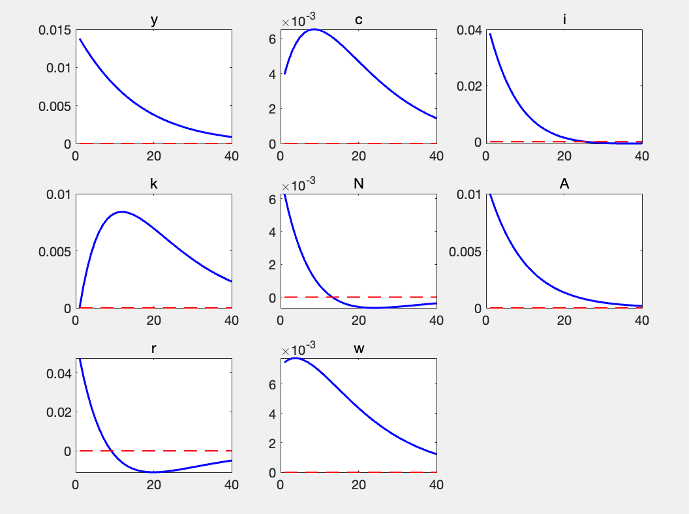
\includegraphics[width=0.8 \linewidth]
			    {pic/1_13.png}
	%		    \caption{二.4}
			  \end{center}
			\end{figure}
		\item 模拟时间序列示意图
			\begin{figure}[H]
			  \begin{center}
			    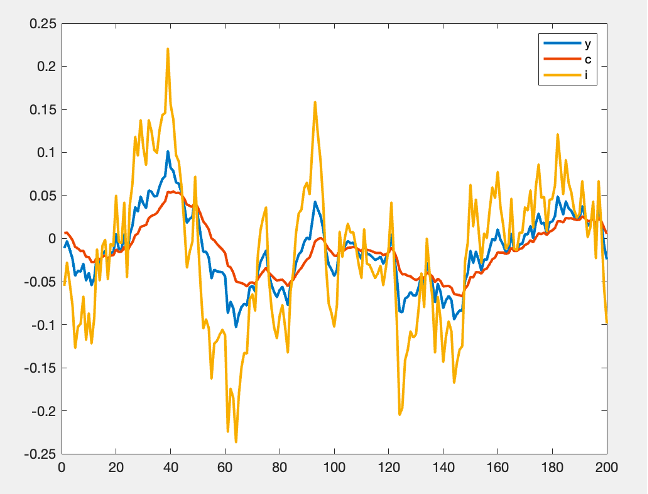
\includegraphics[width=0.8 \linewidth]
			    {pic/1_14.png}
	%		    \caption{二.4}
			  \end{center}
			\end{figure}
			方差为:$$\left[\begin{array}{cccccccc}0.0015 & 0.0009 & 0.0061 & 0.0001 & 0.0081 & 0.0010 & 0.0005 & 0.0014\end{array}\right]$$
			协方差矩阵为:$$\left[\begin{array}{cccccccc}0.0015 & 0.0010 & 0.0028 & 0.0003 & 0.0013 & 0.0012 & 0.0009 & 0.0011 \\0.0010 & 0.0009 & 0.0015 & 0.0001 & -0.0001 & 0.0009 & 0.0005 & 0.0011 \\0.0028 & 0.0015 & 0.0061 & 0.0008 & 0.0051 & 0.0020 & 0.0018 & 0.0013 \\0.0003 & 0.0001 & 0.0008 & 0.0001 & 0.0009 & 0.0002 & 0.0002 & 0.0000 \\0.0013 & -0.0001 & 0.0051 & 0.0009 & 0.0081 & 0.0004 & 0.0012 & -0.0010 \\0.0012 & 0.0009 & 0.0020 & 0.0002 & 0.0004 & 0.0010 & 0.0007 & 0.0011 \\0.0009 & 0.0005 & 0.0018 & 0.0002 & 0.0012 & 0.0007 & 0.0005 & 0.0005 \\0.0011 & 0.0011 & 0.0013 & 0.0000 & -0.0010 & 0.0011 & 0.0005 & 0.0014 \end{array}\right]$$
			自相关系数矩阵为:
			$$\left[\begin{array}{cccccccc}1.0000 & 0.9035 & 0.9136 & 0.7107 & 0.3780 & 0.9679 & 0.9779 & 0.7717 \\0.9035 & 1.0000 & 0.6512 & 0.3406 & -0.0553 & 0.9822 & 0.7939 & 0.9698 \\0.9136 & 0.6512 & 1.0000 & 0.9353 & 0.7217 & 0.7821 & 0.9785 & 0.4466 \\0.7107 & 0.3406 & 0.9353 & 1.0000 & 0.9200 & 0.5110 & 0.8421 & 0.1011 \\0.3780 & -0.0553 & 0.7217 & 0.9200 & 1.0000 & 0.1331 & 0.5633 & -0.2970 \\0.9679 & 0.9822 & 0.7821 & 0.5110 & 0.1331 & 1.0000 & 0.8939 & 0.9068 \\0.9779 & 0.7939 & 0.9785 & 0.8421 & 0.5633 & 0.8939 & 1.0000 & 0.6217 \\0.7717 & 0.9698 & 0.4466 & 0.1011 & -0.2970 & 0.9068 & 0.6217 & 1.0000\end{array}\right]$$
		\item 均值:
			$$\left[\begin{array}{c}0.1321 \\ -0.2020 \\ -1.1265 \\ 1.8693 \\ -1.0260 \\ 0 \\ -3.8918 \\ 0.6473\end{array}\right]$$
			方差:
			$$\left[\begin{array}{c}0.0015 \\ 0.0009 \\ 0.0060 \\ 0.0001 \\ 0.0080 \\ 0.0010 \\ 0.0005 \\ 0.0014\end{array}\right]$$
			标准差:
			$$\left[\begin{array}{c}0.0390 \\ 0.0292 \\ 0.0774 \\ 0.0114 \\ 0.0895 \\ 0.0319 \\ 0.0229 \\ 0.0378\end{array}\right]$$
			协方差矩阵
			$$\left[\begin{array}{cccccccc}0.0015 & 0.0010 & 0.0028 & 0.0003 & 0.0013 & 0.0012 & 0.0009 & 0.0011 \\0.0010 & 0.0009 & 0.0015 & 0.0001 & -0.0001 & 0.0009 & 0.0005 & 0.0011 \\0.0028 & 0.0015 & 0.0060 & 0.0008 & 0.0050 & 0.0019 & 0.0017 & 0.0013 \\0.0003 & 0.0001 & 0.0008 & 0.0001 & 0.0009 & 0.0002 & 0.0002 & 0.0000 \\0.0013 & -0.0001 & 0.0050 & 0.0009 & 0.0080 & 0.0004 & 0.0012 & -0.0010 \\0.0012 & 0.0009 & 0.0019 & 0.0002 & 0.0004 & 0.0010 & 0.0007 & 0.0011 \\0.0009 & 0.0005 & 0.0017 & 0.0002 & 0.0012 & 0.0007 & 0.0005 & 0.0005 \\0.0011 & 0.0011 & 0.0013 & 0.0000 & -0.0010 & 0.0011 & 0.0005 & 0.0014 \end{array}\right]$$
			自相关矩阵:
			$$\left[\begin{array}{cccccccc}1.0000 & 0.9036 & 0.9136 & 0.7104 & 0.3772 & 0.9679 & 0.9779 & 0.7721 \\0.9036 & 1.0000 & 0.6514 & 0.3405 & -0.0558 & 0.9823 & 0.7941 & 0.9699 \\0.9136 & 0.6514 & 1.0000 & 0.9352 & 0.7212 & 0.7821 & 0.9784 & 0.4470 \\0.7104 & 0.3405 & 0.9352 & 1.0000 & 0.9198 & 0.5108 & 0.8419 & 0.1012 \\0.3772 & -0.0558 & 0.7212 & 0.9198 & 1.0000 & 0.1325 & 0.5626 & -0.2973 \\0.9679 & 0.9823 & 0.7821 & 0.5108 & 0.1325 & 1.0000 & 0.8940 & 0.9070 \\0.9779 & 0.7941 & 0.9784 & 0.8419 & 0.5626 & 0.8940 & 1.0000 & 0.6221 \\0.7721 & 0.9699 & 0.4470 & 0.1012 & -0.2973 & 0.9070 & 0.6221 & 1.0000 \end{array}\right]$$
	\end{enumerate}
\end{answer}

\begin{problem}
	\textbf{二、在标准的 RBC模型中分析消费习惯和劳动供给的跨期替代弹性。}假设家庭的单期效用函数为:
	\[
	u\left(c_{t},c_{t-1},n_{t}\right)=\log\left(c_{t}-\eta c_{t-1}\right)-a\frac{n_{t}^{1+\gamma}}{1+\gamma},\quad0<\eta<1.
	\]
	预算约束为:$c_{t}+k_{t+1}-\left(1-\delta\right)k_{t}\leq A_{t}k_{t}^{\alpha}n_{t}^{1-\alpha}$。其中:$\ln A_{t}=\rho\ln A_{t-1}+\varepsilon_{t}$。
	\begin{enumerate}
		\item 请写出模型的均衡条件。 
		\item 求解模型的稳态。 
		\item 写出模型一阶条件的对数线性化系统。 
		\item 假设稳态年利率为4\%,年折旧率为10\%。资本的收入份额为1/3,$\eta=0.5$,$\rho=0.9$。据此设定模型的参数值,分析脉冲反应函数,并根据$\eta$在$\{0,\ 0.5,\ 0.8,\ 0.9,\ 0.99\}$这几个取值下模型动态的变化讨论该参数的作用。(本小题需要使用MATLAB和Dynare软件包。)
		\item 当$\gamma$值在$[0.5,2.5]$之间(取100个点)变化时,模型鞍点路径中劳动供给的系数如何变化,作图并讨论其经济含义。(本小题需要使用MATLAB和Dynare软件包。)
	\end{enumerate}
	\
\end{problem}
\begin{answer}
	\begin{enumerate}
		\item 家庭最大化终身效用的折现值:
			$$
			\begin{array}{c}
				\max_{c_{t},n_t, k_{t+1}}\ E_{0} \sum_{t=0}^{\infty} \beta^{t}\left[\ln \left(c_{t}-\eta c_{t-1}\right)-\alpha \frac{n_{t}^{1+r}}{1+r}\right] 
				\\
				\text{s.t.}\ C_{t}+g_{Z} k_{t+1}=\left(1+r_{t}\right) k_{t}+w_{t} n_t
			\end{array}
			$$
			拉格朗日函数为:
			$$
			\mathcal{L}=E_{0}\sum_{t=0}^{\infty}{
			\beta^t
			\{
			\ln{\left(c_{t}-\eta c_{t-1}\right)}-\alpha \frac{n_{t}^{1+r}}{1+r}+\lambda_{t}[\left(1+r_{t}\right) k_{t}+w_t n_t-c_{t}-g_{Z} k_{t+1}]
			\}
			}
			$$
			均衡条件:
			\begin{itemize}
				\item 对$c_t$求导:$\lambda_t=\frac{1}{c_t-\eta c_{t-1}}-\frac{\eta \beta}{c_{t+1}-\eta c_t}$
				\item 对$n_t$求导:$\lambda_{t}=\frac{\alpha n_{t}^{\gamma}}{w_{t}}$
				\item 对$k_{t+1}$求导:$\beta \lambda_{t+1}\left(1+r_{t+1}\right)=\lambda_{t} g_{Z}$
			\end{itemize}
			厂商最大化利润:
			$$
			\max_{k_t, n_t} A_{t} k_{t}^{\alpha} n_{t}^{1-\alpha}-\left(r_{t}+\delta\right) k_{t}-w_{t} n_{t}
			$$
			均衡条件:
			$$
			\begin{array}{l}y_{t}=A_{t} k_{t}^{\alpha} n_{t}{ }^{1-\alpha} \\ r_{t}=\alpha \frac{y_{t}}{k_{t}}-\delta \\ w_{t}=(1-\alpha)\frac{y_{t}}{n_{t}}
			\end{array}
			$$
		\item 稳态时:
			$$
			\begin{array}{l}
				n_{t}^{\gamma}=\frac{w}{a} \frac{1-\eta \beta}{(1-\eta)c}
				\\
				g_{Z}=\beta(1+r)
				\\
				y=c+g_{z} k-(1-\delta) k
				\\
				\gamma=\alpha \frac{y}{k}-\delta
				\\
				w=(1-\alpha) \frac{y}{n}
			\end{array}
			$$
			外生变量$A_t$不变,因此$g_Z=1$,$A=1$。
			\begin{itemize}
				\item $r=\frac{g_Z}{\beta}-1$
				\item $\frac{k}{y}=\frac{\alpha}{\gamma+\delta}$
				\item $\frac{c}{y}=1-(g_Z-1+\delta)\frac{k}{y}$
				\item $y=A k^{\alpha} n^{1-\alpha} \Rightarrow(\frac{k}{y})^\alpha(\frac{n}{y})^{1-\alpha}=1\Rightarrow\frac{n}{y}=(\frac{k}{y})^{-\frac{\alpha}{1-\alpha}}$
				\item $w=(1-\alpha)\frac{y}{n}$
				\item $n^{\gamma}=\frac{w}{a}\frac{1-\eta \beta}{(1-\eta)c}\Rightarrow(\frac{n}{y}\cdot y)^\gamma=\frac{1-\alpha}{\alpha}\cdot\frac{y}{n}\cdot\frac{1-\eta\beta}{1-\eta}\cdot\frac{y}{c}\cdot\frac{1}{y}$,带入$\frac{n}{y}$和$\frac{c}{y}$可解得$y$。
			\end{itemize}
		\item $$
			\begin{array}{c}
				\frac{a \cdot n_{t}^{\gamma}}{w_{t}}=\frac{1}{c_{t}-\eta c_{t-1}}-\frac{\eta \beta}{c_{t+1}-\eta c_{t}} 
				\\ \frac{n_{t}^{\gamma}}{w_{t}} g_{Z}=\beta \frac{n_{t+1}^{\gamma}}{w_{t+1}}\left(1+r_{t+1}\right) 
				\\ y_{t}=A_{t} k_{t}^{\alpha} n_{t}^{1-\alpha} 
				\\ r_{t}=\alpha \frac{y_{t}}{k_{t}}-\delta 
				\\ w_{t}=(1-\alpha) y_{t} / n_{t} 
				\\ \ln A_{t+1}=P_{A} \ln A_{t}+\epsilon_{A t} 
				\\ i_t=g_{t} k_{t+1}-(1-\delta) k_{t} 
				\\ y_{t}=C_{t}+i_{t}
			\end{array}
			$$
			对数线性化系统:
			$$
			\begin{array}{c}
				\gamma \hat{n}_{t}-\hat{w}_{t}=\frac{\eta \beta \hat{c}_{t-1}-\left(1+\eta^{2} \beta\right) \hat{c_{t}}+\eta \hat{c_{t-1}}}{(-\eta \beta)(1-\eta)} 
				\\
				\gamma{n_{t}}-\hat{w}_{t}=r \hat{n}_{t+1}-\hat{w}_{t+1}+\frac{\gamma}{1+\gamma} \hat{r}_{t+1}
				\\
				\hat{y}_{t}=\hat{A}_{t}+\alpha \hat{k}_{t}+(1-\alpha) \hat{n}_{t}
				\\
				\frac{\gamma}{\gamma+\delta} \hat{r}_{t}=\hat{y}_{t}-\hat{k}_{t}
				\\
				\hat{w}_{t}=\hat{y}_{t}-\hat{n}_{t}
				\\
				\hat{A}_{t+1}=P_{A} \hat{A}_{t}+\epsilon_{A_{t+1}}
				\\
				\hat{\delta}_{t}=\frac{g_{Z}}{g_{Z}-1+\delta} \hat{k}_{t+1}-\frac{1-\delta}{g_{z}-1+\delta} \hat{k}_{t}
				\\
				\hat{y}_{t}=\frac{c}{y} \hat{c}_{t}+\frac{i}{y} \hat{i}_{t} 
			\end{array}
			$$
		\item 随着$\eta$增大,产出、消费、资本存量对技术冲击的反应变得越来越平缓。技术对劳动的冲击由正转负。当$\eta=0.8$时,冲击的影响最为缓和;而当$\eta=0.99$时,技术对消费的影响非常平缓,不再呈现驼峰状。从效用函数的角度看,$\eta$度量了上一期消费负效应的程度,$\eta$的值越大,消费者的消费习惯越稳固,其消费行为也越一致,也就是需要更多的当期消费来匹配过去的消费习惯。当$\eta=0.99$时,消费者的消费习惯十分稳固,对技术冲击对反应也就不再敏感。
		\begin{figure}[H]
		  \begin{center}
		    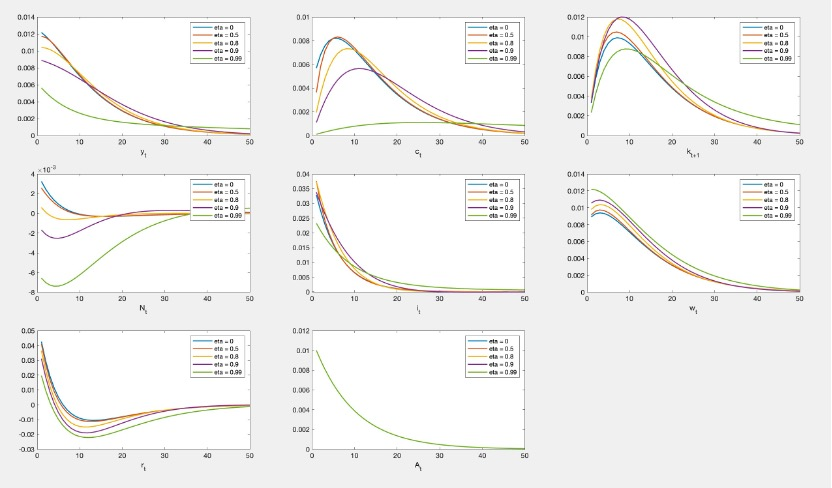
\includegraphics[width=0.8 \linewidth]
		    {pic/2_4.jpg}
%		    \caption{二.4}
		  \end{center}
		\end{figure}
		\item 技术和消费的系数大于0,资本存量的系数小于0,随着γ的增大,三个系数的绝对值均减小,说明技术冲击对劳动供给的影响越来越小。由于$\lambda=\frac{\alpha n^\gamma}{w}$,因此$\frac{1}{\gamma}=\frac{d(\ln n)}{d{\ln w}}$为劳动的弹性,随着$\gamma$增大,劳动的供给弹性变小,劳动对工资的敏感程度降低,所以面对技术冲击时家庭不愿意改变劳动供给,系数绝对值也就减小了。
		\begin{figure}[H]
		  \begin{center}
		    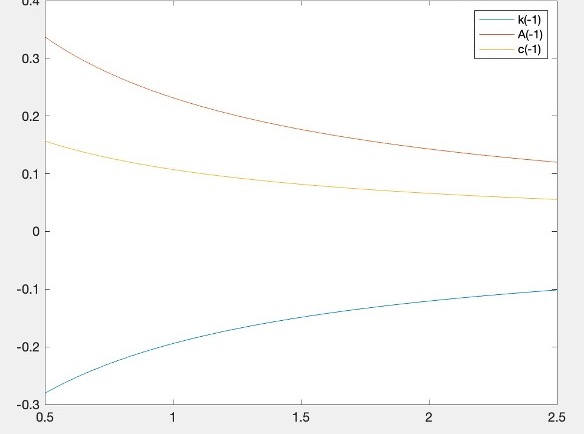
\includegraphics[width=0.8 \linewidth]
		    {pic/2_5.jpg}
%		    \caption{2.5}
		  \end{center}
		\end{figure}
	\end{enumerate}
\end{answer}

\begin{problem}
	\textbf{三、考虑 Calvo 定价模型。}已知厂商$i$面临的产品需求函数为$Y_{i t}=\left(\frac{P_{i t}}{P_{t}}\right)^{-\varepsilon} Y_{t}$。假设厂商每期可以选择最优价格的概率为$1-\gamma$,从而厂商的最优定价问题为:
	\[
		\max _{p_{i t}} E_{t} \sum_{s=0}^{\infty} \gamma^{s} \Lambda_{t+s}\left[\frac{P_{i t}}{P_{t+s}}-m c_{t+s}\right] Y_{i t+s}
	\]
	其中$\Lambda_{t+s} \equiv \beta^{s} \frac{C_{t}}{C_{t+s}}$表示随机折现因子。
	\begin{enumerate}
		\item 请写出厂商定价的一阶条件。
		\item 把最优定价的表达式写为$P_{i t}^{*}=\frac{\varepsilon}{\varepsilon-1} \frac{X_{1 t}}{X_{2 t}}$,写出$X_{1t}$和$X_{2t}$的迭代方程形式,并验证当$\gamma=0$时,$P_{i t}^{*}=\frac{\varepsilon}{\varepsilon-1} m c_{i t} P_{t}$。
	\end{enumerate}
	\
\end{problem}
\begin{answer}
	\begin{enumerate}
		\item 厂商最优定价问题
			$$\max _{p_{i t}} E_{t} \sum_{s=0}^{\infty} \gamma^{s} \beta^{s} \frac{c_{t}}{c_{t+s}}\left[\frac{P_{i t}}{P_{t+s}}-m C_{t+s}\right] \cdot\left(\frac{P_{i t}}{P_{t}}\right)^{-\varepsilon} Y_{t+s}$$
			一阶条件:
			$$E_{t} \sum_{s=0}^{\infty}(\gamma \beta)^{s} \frac{c_{t}}{c_{t+s}} \cdot P_{t+s}^{\varepsilon}\left[(1-\varepsilon) \frac{P_{i t}}{P_{t+s}}+\varepsilon m c_{t+s}\right] Y_{t+s}=0$$
		\item 将一阶条件改写为$P_{i t}^{*}=\frac{\varepsilon}{\varepsilon-1} \frac{X_{1 t}}{X_{2 t}}$
			$$P_{0 t}^{*}=\frac{\varepsilon}{\varepsilon-1} \frac{E_{t} \sum_{s=0}^{\infty}(\gamma \beta)^{s} c_{t} \cdot P_{t+s}^{c} \cdot m Y_{t+s}}{E_{t} \sum_{s=0}^{\infty}(\gamma \beta)^{s} \frac{c_{t}}{c_{t+s}} P_{t+s}^{e-1} Y_{t+s}}$$
			因此,
			$$X_{1 t}=E_{t} \sum_{s=0}^{\infty}(\gamma \beta)^{s} c_{t} \cdot P_{t+s}^{c} \cdot m Y_{t+s}=c_{t}P_{t}^{\varphi} m Y_{t}+\gamma \beta X_{1t+1}$$
			$$X_{2 t}=E_{t} \sum_{s=0}^{\infty}(\gamma \beta)^{s} \frac{c_{t}}{c_{t+s}} P_{t+s}^{e-1} Y_{t+s}=P_{t}^{\varphi-1} Y_{t}+\gamma \beta X_{2 t+1}$$
			当$\gamma=0$时,
			$$
			P_{i t}^{*}=\frac{\varphi}{\varphi-1} \cdot \frac{c_{i t} \cdot P_{t}^{\varphi} \cdot m Y_{t}}{\frac{c_{t}}{c_{t}} \cdot P_{t+s}^{\varphi-1} Y_{t}}=\frac{\varphi}{\varphi-1} \cdot c_{i t} m P_{t}
			$$
	\end{enumerate}
\end{answer}
\end{CJK*}
\end{document}